%\subsection{Modeling\label{sec:modeling}}
%%The modeling steps builds upon the previous data preprocessing and feature selection process. 
%%This assumes the analyst already has an understanding about the data and prepared it for analysis.
%%Further, he took care of feature generation and feature selection in order to represent the data accordingly. 
%%During this step, systems support the analyst with e.g. subspace exploration, training set modification, parameter tuning. \cite{Lu:2017}\\
%An popular approach for general time series analysis is from Buono et al. \cite{buono:2005} and focuses explicitly on automatically finding similar patterns compared to a user specified pattern.
%The system was built upon \textit{TimeSearcher} proposed by Hochheiser and Shneiderman \cite{Hochheiser:2004}, which concentrates on high usability even for users without specialized skills such as in statistics.
%%Based on their idea, Buono et al. continued with using timeboxes, i.e. rectangular regions that filter the data and reduce the scope of each search.
%%Their updated version adds another variant for pattern search in the remaining data. 
%%Further, they also allow users to work with long time series of multiple heterogeneous variables. 
%However, these two version of \textit{TimeSearcher} are more interested in data exploration and consequently would be located either in the data preprocessing or as supporting tool in the feature engineering step. 
%%For data exploration the user is initially presented with a multivariable time series viewer, which allows to visually analyze multiple variables in parallel on different levels-of-detail.
%%In order to detect reoccurring and similar patterns, the user highlights a found pattern within the time series and the system uses a similarity-based search to find other occurrences. 
%%Therefor, the search space can be limited to only interesting areas.
%%The initial matches of the given pattern can afterwards be refined to support the analysis goal better. 
%%This process of returning many results and consequently enable the user to reduce the outcome to his/her liking, can also be found in spatiotemporal approaches (\autoref{sec:spatiotemp}), esp. in the template driven approach of \cite{malik:2014}.
%%Moreover, \textit{TimeSearcher} also provides different data transformations to match patterns more easily. 
%%One drawback of the system is that it cannot deal with missing data points and pattern matching is very depended on the user's chosen parameters.
%For modeling the updated version of \textit{TimeSearcher} by Buono et al. \cite{buono:2007} is of greater interest.  
%For its prediction, it resorts on the similarity-based approach, which was used in the previous version \cite{buono:2005} to detect time series with similar behavior.
%In order to provide the analyst with an better overall understanding of the selected subset of time series, the system offers a summarized view based on a river plot, which also incorporates confidence bands (bottom right of \autoref{fig:timesearcher}).
%The actual prediction is computed by extrapolating only those time series, which were identified as similar to the target time series.
%%As in \cite{buono:2005} the system is meant for users without statistical knowledge.
%In order enable the analyst to select a better model, the simultaneous preview interface allows to compare multiple parameter choices as well as different modeling techniques, such as smoothing, in parallel (\autoref{fig:timesearcher}). 
%Given the data-driven nature of the system, this requires the analyst to provide larger datasets compared to a model-driven approach.
%However, the simultaneous preview interface simplifies the modeling process and makes it accessible to untrained users and allows experienced analysts to get a better insight.
%
%\begin{figure}[tb]
%	\centering
%	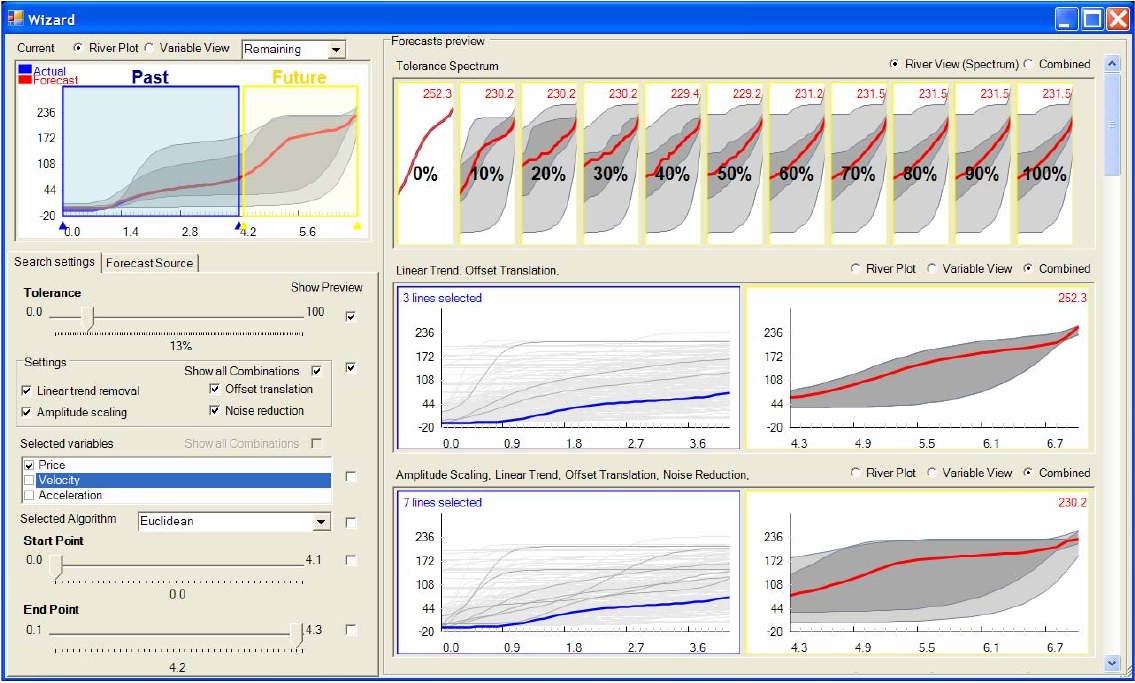
\includegraphics[width=\columnwidth]{TimeSearcher}
%	\caption{TimeSearcher's \cite{buono:2007} simultaneous preview interface
%	}
%	\label{fig:timesearcher}
%\end{figure}
%
%In practical scenarios the requirement to have large amounts of data points can often be a problem, which makes the systems \cite{Hochheiser:2004, buono:2005, buono:2007} less valuable.
%Consequently, a model-driven system, which requires less data points, is preferred.
%The approach of \cite{ichikawa:2002} could be seen as such system as it utilizes external simulations models.
%However, it is not supporting the modeling process and is therefore only seen as system for result exploration.
%On the other hand, \textit{TiMoVA} a system, which explicitly provides model parameter selection was proposed from B{\"o}gel et al. \cite{boegl:2013}.
%The system is designed after the Box Jenkins method and is only supporting the model specification and selection process.
%For model specification, i.e. selection of an appropriate model type and its order, they provide autocorrelation function and partial autocorrelation function plots.
%These plots are also utilized by the analyst to select the model's parameters.
%A big drawback of the system are the assumptions about the preprocessed data. 
%It requires a time series without missing values and only supports univariate analysis.


%\subsection{Result Exploration and Validation\label{sec:exploration}}
%Subsequent to the creation of the model, the analyst wants to explore the results/predictions and eventually compare the performance between several models. 
%Therefore, system are often highly interactive to provide the analyst as much freedom as possible.\cite{Lu:2017}\\
%An older Visual Analytics approaches is from Ichikawa et al. \cite{ichikawa:2002}.
%They wanted to enable analysts to predict multiple daytime stock prices and simultaneously visualize a set of predictions from different simulation systems. 
%This means, unlike other systems, their system only supports result exploration and/or model selection by efficiently visualizing a vast amount of predictions.
%As a consequence, the visualization includes multiple predictions for multiple stocks. 
%One major finding was, visualizing multivariate predictions in a 3-dimensional space creates high levels of occlusion, thus, it is not suitable.
%Instead, the system utilizes line charts with cluttering control and color charts with level-of-detail control. 
%%The line charts support multivariate scaling, i.e. the time axis can be scaled differently to focus on certain areas, e.g. areas with higher discrepancies of the simulations.
%%Further, the lines are colored differently, depending on the amount of overlap/uniform predictions.
%The color chart tries to reduce the complexity of all simulations by clustering similar predictions and reducing the time series to its key elements, i.e. the overall trends of each cluster.
%This allows the analyst to detect discrepancies between the clusters.
%Further, he is able to compare specific predictions with the overall trend. 
%%The color chart is composed of horizontal color-bands for each prediction, whereas a vertical color band can be seen as a period in time. 
%%In order to improve the visualization, the different color-bands are cluster based on the user-specified level-of detail. 
%%This results in a smaller amount of horizontal color-bands where the individual properties are diminished. 
%%In the workspace the above plots can be displayed with different axis.
%For additional comparison, the systems workspace visualizes a set of predictions for different parameter ranges (e.g. sales organizations) as well as different stocks.
%Consequently, the user can detect trends concerning the whole stock market.  
%However, due to the amount of simulations displayed, it can be hard to extract specific information.
%
%During the evaluation of \textit{TiMoVA} \cite{boegl:2013}, they found that an actual prediction functionality would provide additional value for the analyst.
%Therefor, they included a result exploration and validation functionality.
%This allows the analyst to adjust different model parameters and see the changes in the corresponding prediction visualizations, which gives him feedback about the adequateness about the chosen model. 
%Similar to \cite{buono:2007}, the prediction is incorporated with confidence bands to express the models certainty. 
%Additionally, they specifically visualize the difference of true and predicted values for each data point as well as the direction (positive or negative).
%This gives the analyst a quick overview if the model is constantly over- or underestimating the time series as well as how long and often this occurs.

%One goal in time series analysis is detecting patterns.
%These patterns help analysts to better understand their data and enables them to formulate improved hypotheses for future developments. 
%Further, they allow analysts to detect unusual occurrences, which makes it possible to spot undesired behaviors in advance and react accordingly. 
%Such anomalies can include fraud attempts, higher server loads or bad configurations of manufacturing machines.\\

%However, in a practical environment it is often necessary to evaluate multiple time series in parallel or deal with multidimensional input variables.
%In order to solve these problems, Visual Analytics approaches for simple time series are not sufficient anymore.\\ 

%\subection{Data Correlations}

%A more specialized data-driven Visual Analytics approach was proposed from Xie et al. \cite{Xie:2014}.
%The difference to other approaches can be found in the application area of customer-to-customer e-transaction time series. 
%The time series consists of transactions between the a seller and a buyer.
%However, the commodities as well as the buyer can vary greatly.
%Finding patterns in such time series helps analysts to understand temporal and contextual connections between multiple transactions of one seller, e.g. high number of transactions with same seller/ with same commodity.
%This can be extended to gain an understanding of the overall selling process or identifying fake transactions.
%For analysis the system employs a iterative process consisting of two main Visual Analytics components, an overview component and a detail component.
%The overview component proposes possible salient transactions. 
%Therefor, a decision tree learner calculates a saliency score for each transaction and a certain analysis task.
%This learner addresses basic features (e.g. commodity, order amount), textual features (e.g. sensitive words in comments) and temporal features (e.g. transaction amount of seller within on time period).
%The latter is difficult to address by a decision tree, hence the systems harnesses the transaction frequency of a seller in a user defined time interval.
%Consequently, the saliency scores are displayed in a time-of-saliency map with an user adjustable level-of-detail. 
%The detailed view is used to gain more insight on specific transactions, which were selected by the user in the overview.
%For visualization, they introduce a musical notation inspired visual metaphor, called KnotLines (\autoref{fig:knotlines}).
%The amount of transactions in one section (e.g. books) defines the size of the corresponding note head, where missing values are explicitly marked to catch the attention of an analyst.
%For each time interval the sections' heads are placed on the same note stem, where the length represents the total payment per seller and per time interval.  
%In order to capture the relationship over multiple time intervals, the stems of one seller are connected by beams.
%This view enables the analyst to observe multiple attributes as well as temporal and contextual correlations of transactions and find salient transactions.
%The identified salient transactions are fed back to decision tree learner, which changes the predictions of the unknown transactions.
%A big drawback of the initial computation of saliency values is the need for training data. 
%Analysts are required to annotate features of training transactions, unlike most other approaches introduced in this survey, which do not require this additional step. 

%\begin{figure}[tb]
% \centering
% 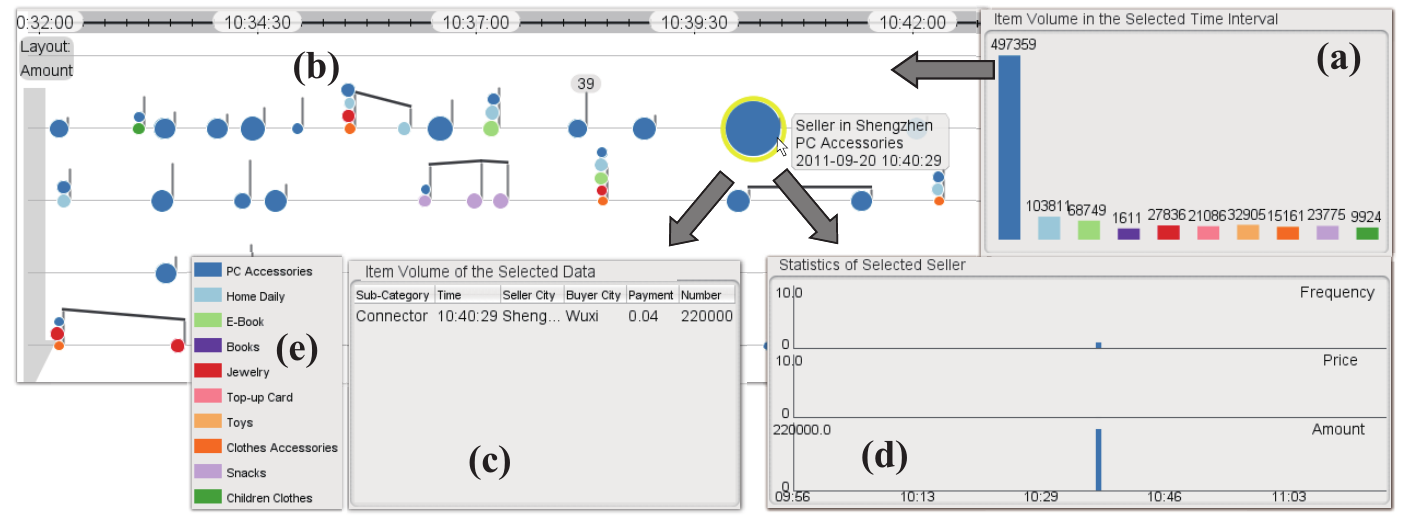
\includegraphics[width=\columnwidth]{KnotLines}
% \caption{KnotLine view from \cite{Xie:2014}. (a) Bar chart for the number of commodities in different categories. (b) The big knot indicates an unusually large number of commodities in a transaction. (c) Detailed information. (d) Statistical information. (e) Sales category legend.
% 	}
% \label{fig:knotlines}
%\end{figure}
%
%Similar to \cite{Xie:2014}, another specialized system was recently presented by Steed et al. \cite{steed:2017}.
%Their approach is focused on understanding patterns in log and imagery data collected by 3D printers, which is highly irregular, includes missing values and has a high complexity in general.
%Unlike the other systems, this Visual Analytics tool is designed from an manufacturing standpoint to discover patterns related to defects and system performance issues, optimizations to avoid defects and increasing production efficiency.
%The visualization of the system is based on the visual information seeking strategy.
%Therefor, the system provides different charts for each variable with individual level-of-detail control and filtering including an interactive statistical view (\autoref{fig:falcon}). 
%They also provide a new visualization technique, called waterfall visualization, to combine overview and detailed view, which is similar to the idea of color charts by \cite{ichikawa:2002}
%Further, a comparative view is provided to analyze different variables of multiple configurations, which also includes pattern matching capabilities. 
%With the application of information scent, the system encodes quantitative values from similarity and statistical methods in the visualization in order to highlight relationships and reduce the search space. 
%From an operational point of view, the system offers, similar to \cite{Xie:2014}, user driven analysis and helps to detect and highlight univariate and multivariate patterns from different angles.
%Technologically, the system is bin based, each bin contains a small subset of data points and the corresponding descriptive statistics. 
%Through the aggregation of bins, a higher level-of-detail abstraction can be achieved. 
%The above parts of the system can be applies well to other problem ares, however they also included visualizations specifically for the analysis of 3D printer data.
%One of those is a segmented time series view, which partitions a selected time series of a variable and also visualizes the images of the printing process next to it. 
%By providing a reference time series, the system computes the similarity/dissimilarity of both series.
%Another feature specifically for 3D printers is the segmentation based on the build height as well as porosity detection.
%Whereas, these specific features provide important information for this use case, they make the system less generic and applicable to other areas. 
%Further, the system currently does not support provenance information and the similarity/dissimilarity methods are limited to the segmented time series view.

%\begin{figure}[tb]
%	\centering
%	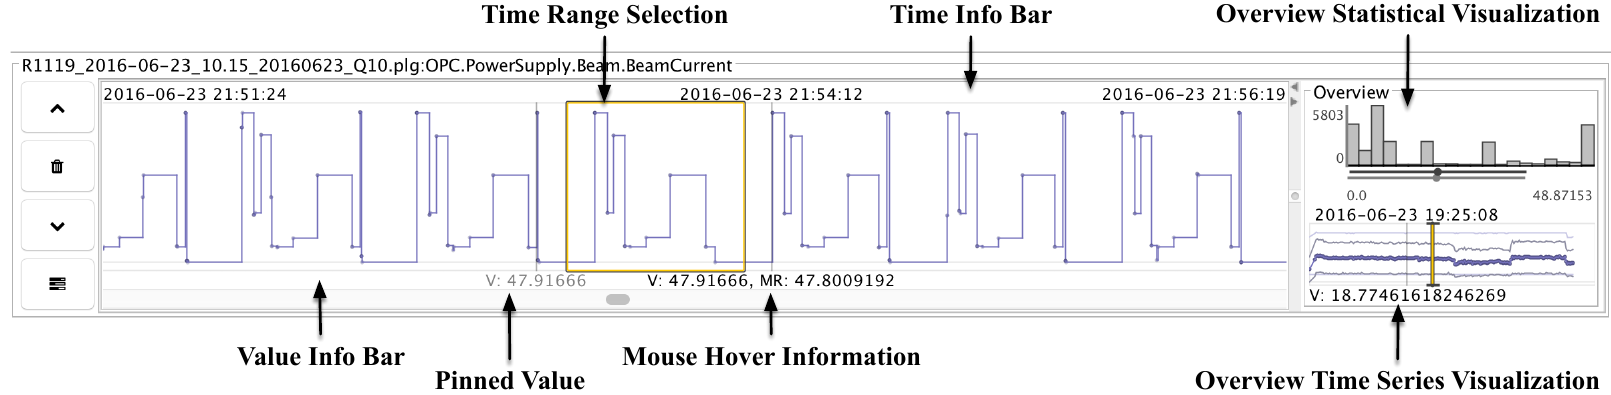
\includegraphics[width=\columnwidth]{Falcon}
%	\caption{Time series visualization of one variable from \cite{steed:2017}
%	}
%	\label{fig:falcon}
%\end{figure}
%
%Other application specific approaches involve pattern detection within patient treatment plans \cite{Gschwandtner:2011} or hypothesis generation for climate research \cite{Kehrer:2008}.
%Whereas, the latter can also be seen as spatiotemporal as it tries to detect regions in the atmosphere, which indicate climate change.
%Similar to \cite{Xie:2014}, Janetzko et al. \cite{janetzko:2014} focuses specifically on anomaly detection.
%However, the underlying time series is based on server power consumption.
%In the same application context is the system of McLachlan et al. \cite{McLachlan:2008}. 
%Their analytics tool was developed for system management and is also viable for large time series, i.e. hundreds of parameters across thousands of network devices.
%Other multivariate systems, such as \cite{ichikawa:2002, buono:2005, buono:2007}, are often not able to present these amounts clearly.
%The application of \cite{steed:2017} is one of the few to provide similar capacity, although a different application area. 
%%\subsection{Peak Preservation \label{subsec:peak}}
%Time series prediction with peak preservation poses a similar problem as pattern and anomaly detection. 
%%However, preserving peaks for prediction can be seen as an additional step. 
%The identified patterns/peaks need to be included in the systems forecast.
%%The application areas for such systems is also differing from trend based predictions, which try to smooth and generalize to have a more consistent prediction. 
%%However, for example when analyzing power consumption time series in data centers, it is important to preserve peaks and their patterns.
%An systems which also includes this additional step in the prediction process is from Hao et al.\cite{Hao:2011, Hao:2009}.
%They applied an automated peak preserving smoothing method in order to reduce noise and get a more reliable prediction as well as retain the seasonality of the data.
%Thereby, the analyst is able to determine the influence of more recent measurements, i.e. how far back in time seasonality is considered in the smoothing process. 
%Otherwise, the system is comparable to \cite{buono:2007}.
%This idea is inherited in \cite{Hao:2012}, where the peak preservation is combined with an automated motif/pattern detection, which includes detecting overlapping patterns. 
%Similar to \cite{buono:2007}, depending on the user's preference, the detected patterns can be aggregated to increase their significance.